\chapter{Tessellation Service}

\section{Objective of the Tessellation Service}
\label{sec5_objective}
The objective of the TS is to provide a service that extracts image regions annotated by the AS to create samples for the training of a NN\footnote{
	Compare subsection \ref{sec2_learning}
}. In this context, "extraction" describes the process of creating sub images of the original image, which contain all of the annotated ROI and as little of anything else as possible. Additionally, the correspondence with the associated region label must be kept. The AS uses \emph{regions}\footnote{
	Compare subsection \ref{sec4_region}
} to describe ROIs. Those regions are persisted in a JSON file.

Therefore, the TS has 2 objectives:
\begin{enumerate}[(1)]
	\item parse a JSON file and acquire its region data
	\item extract ROIs based on the acquired region data
\end{enumerate}


\section{Methodology}
\label{sec5_method}
The objective of the TS is to create usable training samples for NNs, as stated in section \ref{sec5_objective}. Depending on the setup, chosen learning method\footnote{
	Compare section \ref{sec2_introNN}
} and purpose of the NN, the requirements imposed on the training samples may vary. Smith demonstrates in \cite{Smith97} exemplary how to train a NN to recognize letters in images of written text by training it with 10x10 pixel grayscale images (256 gray levels/pixel) of letters. Shereena and David introduce a novel content based image retrieval classification method in \cite{Shereena14}, based on color or texture features. Other approaches extract features through the use of mathematical models from the supplied images (such as edges or shapes)\cite{Harvey91}.

Because of those varying requirements, the TS will be capable of producing different output:
\begin{enumerate}[(1)]
	\item Unaltered image of ROI
	\item Resize images to a specific width and height
	\item Approximate ROIs via tessellation
	\item Convert extracted images to grayscale
\end{enumerate}

A user can draw a region's path without any restrictions concerning the pattern, resulting in ROIs that can be of arbitrary shape. Therefore, bounding boxes (BB)\nmc{BB}{Bounding Box}\footnote{
	A BB is a rectangular body, fully enclosing a provided (two dimensional) object of arbitrary shape\cite{Toussaint83}.
} are used for ROI extraction in the cases (1) and (2) (see fig. \ref{fig5_bbExample} for an example).

\begin{figure}[H]
	\begin{center}
		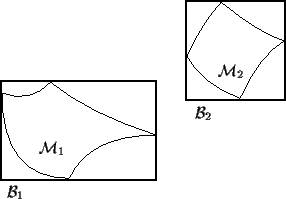
\includegraphics[scale=0.6]{img/bb1.png}
		\caption{Examplary BBs: $B_1$ is BB of $M_1$, $B_2$ is BB of $M_2$ (source: \url{http://www.idav.ucdavis.edu/education/GraphicsNotes/Bounding-Box/Bounding-Box.html})}
		\label{fig5_bbExample}
	\end{center}
\end{figure}

In the case of (1), an ROI's BB is copied pixel by pixel into a new image. The resizing (scaling the output image up or down to the provided pixel values) in the case of (2) makes preprocessing of the BB necessary. This has 2 reasons:
\begin{itemize}
	\item If the aspect ration of the provided width and height is different than the one of the BB, the resulting image will be distorted.
	\item When scaling images down, interpolation can be used, to reduce the information loss of the image\cite{Thevanez00}. This is partially possible when scaling images up as well, e.g. via fractal interpolation, but a non trivial task\cite{Guerdri16}.
\end{itemize}

Therefore, the size of the BB will be adjusted to match the aspect ratio of the provided width and height. If the resulting BB is bigger then the provided width and height, the image will be scaled down and interpolated. If the BB is smaller, it will be scaled up instead of the image. This leads to a bigger area inside the BB that is not part of the ROI, but a pixel ratio of 1:1 between original and extracted image, resulting in no distortion or loss of quality.

Case (3) approximates a ROI by tessellating\footnote{
	\emph{Tessellation} describes the tiling of a plane using one or more geometric shapes with no overlaps or gaps\cite{Clifford09}.
} it into tiles of the provided width and height (see fig. \ref{fig5_tesExample} for an example). Every tile inside the region's enclosing path (or touched by it) is targeted by the extraction. Each tile is extracted into an individual image.

\begin{figure}[H]
	\begin{center}
		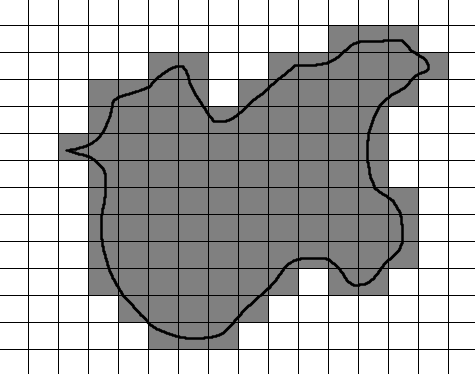
\includegraphics[scale=0.5]{img/tessellation.png}
		\caption{Example of an ROI approximated via tessellation (gray tiles belong to the ROI)}
		\label{fig5_tesExample}
	\end{center}
\end{figure}

Cases (1) - (3) can be combined with (4) to convert the extracted images into grayscale images.

\section{Implementation}
\label{sec5_impl}
The TS is implemented as a python script called \textbf{\emph{TessellationService.py}}\footnote{
	See its GitHub repository for more information: \url{https://github.com/SasNaw/TessellationService}.
}. \emph{OpenSlide} was used to access and read a provided WSI, as in chapters \ref{sec3_cs} (VIPS uses OpenSlide for the same reason\cite{cupitt96}) and \ref{sec4_as}. Additionally, \emph{NumPy}\footnote{
	See \url{http://www.numpy.org/} for more information on NumPy.
} and \emph{OpenCV}(Open Source Computer Vision Library)\nmc{OpenCV}{Open Source Computer Vision Library}\footnote{
	See \url{http://opencv.org/} for more information on OpenCV.
} were used to increase imaging and calculating functionality.

NumPy is a python library for efficient scientific computing, especially regarding operations involving multi-dimensional array objects\cite{Walt11}. Since a lot of image operations are based on the use of matrices, this library was used to increase efficiency.

OpenCV  is an open source computer vision and machine learning software library. It was built to provide a common infrastructure for computer vision applications. It offers numerous functions regarding image processing and machine learning, with a strong focus on real-time computing and efficiency\cite{Bradski08}. Its main purpose in the TS is to create a reference image for the tessellation function\footnote{
	See subsection \ref{sec5_tessellation}
}

The TS can be called over the python interpreter:

\begin{lstlisting}
	$ python TessellationService [input] [params]
\end{lstlisting}

The files which are supposed to be targeted by the extraction process are handed to the TS via the \emph{[input]} argument. This can be
\begin{itemize}
	\item a WSI of proprietary format\footnote{
		Compare subsection \ref{sec2_proprietaryForams}
	}
	\item a DZI
	\item a directory with WSIs and DZIs
	\item a list of all the types mentioned above
\end{itemize}

If a directory is handed to the TS, all subdirectories will be searched as well.

Each WSI and DZI targeted by the TS must have an associated JSON file with annotations created by the AS\footnote{
	Compare chapter \ref{sec4_as}
}. The [input] argument is mandatory.

As mentioned in section \ref{sec5_method}, it might be necessary to create different output images for different purposes. Therefore, the TS has a list of optional parameters to manipulate the created output in order to be applicable to a wider variety of cases (see tab. \ref{tab5_tsParams}). Those parameters are optional. 

\begin{table}[H]
	\begin{center}
		\begin{tabular}{| p{3cm} | p{5cm} | p{3cm} |}
			\hline
			\textbf{name} & \textbf{description} & \textbf{default}\\ \hline
			-h, --help & show help & - \\ \hline
			-f, --force-overwrite & flag to overwrite images with the same name (if not supplied, \emph{"{\textunderscore}copy"} will be added to the image name) & false \\ \hline
			-g, --grayscale & flag to convert images to grayscale images before saving them & false \\ \hline
			-i, --interpolation & choose interpolation method: nearest neighbor, bilinear, bicubic, lanczos  & nearest neighbor interpolation \\ \hline
			-o, --output [directory] & choose output directory (if not provided, the TS will save all extracted images in its own directory) & - \\ \hline
			-r, --resize [width] [height] & resize all output images to the provided [width] and [height] in pixel & - \\ \hline
			-s, --show-tessellated & flag to create window and show stitched image resulting from the tessellation process (only for debugging purposes, see \emph{"-t"}) & false\\ \hline
			-t, --tessellate [width] [height] & tessellate regions into tiles of the provided [width] and [height] in pixels & - \\ \hline
		\end{tabular}
		\caption{Optional parameters for the TS}
		\label{tab5_tsParams}
	\end{center}
\end{table}


\subsection{Extraction process}

The TS expects a list of input arguments. Those arguments will be iterated and their annotated regions extracted from the corresponding JSON file (see fig. \ref{fig5_extractionProcess} for an overview).

After the arguments and parameters are parsed, the script's \texttt{run()} method is called:

\begin{lstlisting}[frame=single, language=python, title=\texttt{run()} from TessellationService.py]
def run(input):
	for element in input:
			# input is folder:
			if(os.path.isdir(element)):
				files_from_dir(element)
			# input is file:
			elif(os.path.isfile(element)):
				regions_from_file(element)
\end{lstlisting}

As stated in section \ref{sec5_method}, valid input are lists of files and folders. Therefore, the individual entries of the input list must be examined. If the current element is a WSI or DZI, the extraction begins right away (see line 8 in \texttt{run()}). If it is a directory, \texttt{files{\textunderscore}from{\textunderscore}dir(dir)} will be called (see line 5 in \texttt{run()}) and search for valid files, including all contained subdirectories:

\begin{lstlisting}[frame=single, language=python, title=\texttt{files{\textunderscore}from{\textunderscore}dir(dir)} from TessellationService.py]
def files_from_dir(dir):
	if not dir.endswith('/'):
		dir = dir + '/'
	contents = os.listdir(dir)
	for content in contents:
		if os.path.isdir(dir + content):
			if not content.endswith('_files'):
				files_from_dir(dir + content)
		else:
			regions_from_file(dir + content)
\end{lstlisting}

After the contents of the directory are received (see line 4 in \texttt{files{\textunderscore}from{\textunderscore} dir(dir)}), they are evaluated further (see line 5 - 10 in \texttt{files{\textunderscore}from{\textunderscore}dir(dir)}). If the input directory contains subdirectories, \texttt{files{\textunderscore}from{\textunderscore}dir(dir)} is called recursively for each one of them, until the end of each directory tree is reached (see line6 - 8 in \texttt{files{\textunderscore}from{\textunderscore}dir(dir)}). Otherwise, the extraction process is started for the detected file (see line 9 - 10 in \texttt{files{\textunderscore}from{\textunderscore}dir(dir)}). Directories ending in \emph{"{\textunderscore}files"} are excluded since they only contain the tiled images for an associated DZI metadata file and a metadata.txt, if they were converted by the CS\footnote{
	Compare chapter \ref{sec3_cs}
} (see line 7 in \texttt{files{\textunderscore}from{\textunderscore}dir(dir)}).

\begin{figure}[H]	
	\begin{center}
		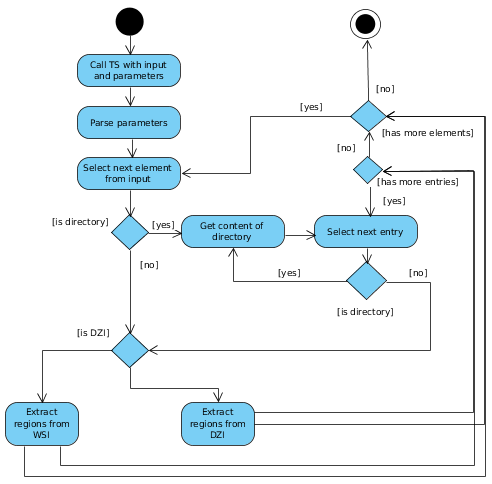
\includegraphics[scale=0.4]{img/ts_run.png}
		\caption{Activity diagram of TS' extraction process}
		\label{fig5_extractionProcess}
	\end{center}
\end{figure}

OpenSlide is used to read a WSI. Since OpenSlide can only wrap an \emph{OpenSlide object} into a DZG\footnote{
	Compare subsection \ref{sec4_openslide}
}, but not read a native DZI\cite{web:openslide}, a different approach was chosen for DZI. Because of this, the implementation for DZI and WSI differs.


\subsubsection{WSI}

\begin{figure}[H]
	\begin{center}
		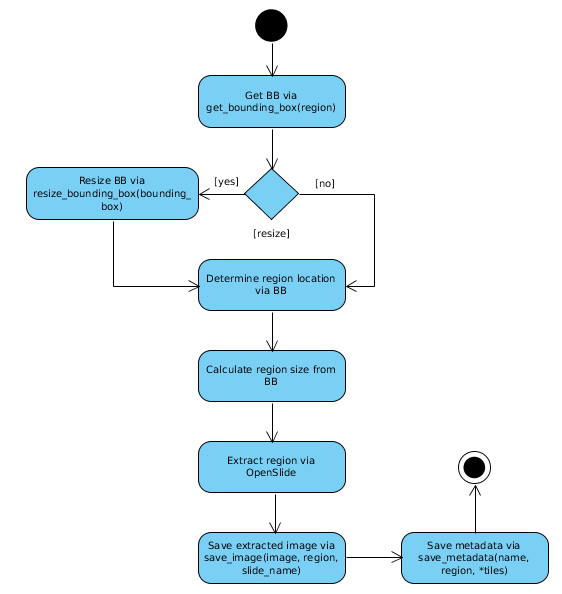
\includegraphics[scale=0.5]{img/ts_wsi_uml.png}
		\caption{Activity diagram of TS' WSI extraction}
		\label{fig5_tsWsiUml}
	\end{center}
\end{figure}


\subsubsection{DZI}

\begin{figure}[H]
	\begin{center}
		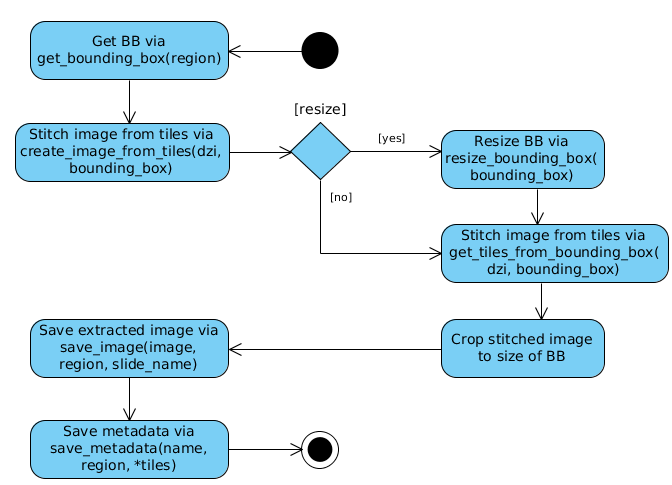
\includegraphics[scale=0.4]{img/ts_dzi_uml.png}
		\caption{Activity diagram of TS' DZI extraction}
		\label{fig5_tsDziUml}
	\end{center}
\end{figure}


\subsection{Tessellation}
\label{sec5_tessellation}

\section{Test}
\subsection{Setup}
\subsection{Result}